%%%%%%%% ICML 2021 EXAMPLE LATEX SUBMISSION FILE %%%%%%%%%%%%%%%%%

\documentclass{article}

% Recommended, but optional, packages for figures and better typesetting:
\usepackage{microtype}
\usepackage{graphicx}
\usepackage{subfigure}
\usepackage{booktabs} % for professional tables
\usepackage{xcolor}
% hyperref makes hyperlinks in the resulting PDF.
% If your build breaks (sometimes temporarily if a hyperlink spans a page)
% please comment out the following usepackage line and replace
% \usepackage{icml2021} with \usepackage[nohyperref]{icml2021} above.
\usepackage{hyperref}

% Attempt to make hyperref and algorithmic work together better:
\newcommand{\theHalgorithm}{\arabic{algorithm}}
% Redefine section commands with colors



\usepackage{xcolor}
\definecolor{imperialblue}{rgb}{0, 0, 0.804}
\definecolor{crimson}{rgb}{0.8627, 0.078, 0.23529}
\definecolor{springgreen}{rgb}{0, 0.5, 0.5}
\definecolor{violet}{rgb}{0.7803, 0.082, 0.52156}
\definecolor{indigo}{rgb}{0.294, 0.0, 0.5098}

% Define new commands for section headings with colors
\newcommand{\csection}[1]{\section{\textcolor{imperialblue}{#1}}}
\newcommand{\csubsection}[1]{\subsection{\textcolor{springgreen}{#1}}}
\newcommand{\csubsubsection}[1]{\subsubsection{\textcolor{violet}{#1}}}
\newcommand{\cparagraph}[1]{\paragraph{\textcolor{crimson}{#1}}}
\newcommand{\csubparagraph}[1]{\subparagraph{\textcolor{indigo}{#1}}}


% Use the following line for the initial blind version submitted for review:
\usepackage{icml2021}

% If accepted, instead use the following line for the camera-ready submission:
%\usepackage[accepted]{icml2021}

% The \icmltitle you define below is probably too long as a header.
% Therefore, a short form for the running title is supplied here:
\icmltitlerunning{\textcolor{violet}{Grading Rubric and Formatting Instructions for ImpCML 2024}}

\begin{document}

\twocolumn[
\icmltitle{\textcolor{black}{Grading Rubric and Formatting Instructions for \\
           Imperial Coursework on Machine Learning (ImpCML 2024)}}

% It is OKAY to include author information, even for blind
% submissions: the style file will automatically remove it for you
% unless you've provided the [accepted] option to the icml2021
% package.

% List of affiliations: The first argument should be a (short)
% identifier you will use later to specify author affiliations
% Academic affiliations should list Department, University, City, Region, Country
% Industry affiliations should list Company, City, Region, Country

% You can specify symbols, otherwise they are numbered in order.
% Ideally, you should not use this facility. Affiliations will be numbered
% in order of appearance and this is the preferred way.
\icmlsetsymbol{equal}{*}

\begin{icmlauthorlist}
\icmlauthor{Firstname Lastname}{Imp}
\end{icmlauthorlist}

\icmlaffiliation{Imp}{Department of Computing, Imperial College London, London, United Kingdom}

\icmlcorrespondingauthor{Firstname Lastname}{first.last@imperial.ac.uk}
\icmlcorrespondingauthor{Eee Pppp}{ep@eden.co.uk}

% You may provide any keywords that you
% find helpful for describing your paper; these are used to populate
% the "keywords" metadata in the PDF but will not be shown in the document
\icmlkeywords{Machine Learning, ICML}

\vskip 0.3in
]

% this must go after the closing bracket ] following \twocolumn[ ...

% This command actually creates the footnote in the first column
% listing the affiliations and the copyright notice.
% The command takes one argument, which is text to display at the start of the footnote.
% The \icmlEqualContribution command is standard text for equal contribution.
% Remove it (just {}) if you do not need this facility.

%\printAffiliationsAndNotice{}  % leave blank if no need to mention equal contribution
\printAffiliationsAndNotice{\icmlEqualContribution} % otherwise use the standard text.

\begin{abstract}
This document provides a basic paper template and submission guidelines.
Abstracts must be a single paragraph, ideally between 4--6 sentences long.
Gross violations will trigger corrections at the camera-ready phase. 
\textcolor{crimson}{This document contains both formatting and grading criteria.}
\end{abstract}

\csection{Grading Rubric}

%Part of the grading for this assignment is, admittedly subjective. While instructors will be lenient on the technical quality of writing, if no effort is shown or understanding is significantly hindered this will affect the resulting marks for the submission. 
The marks for this assignment are broken down as follows: 

\begin{itemize}
    \item \textbf{Writing Quality (5 marks):} The outline of a prototypical submission is given in the submission instructions. This evaluates the clarity, structure, and overall presentation of the submission. Proper grammar, use of technical language, and effective communication are essential.
  
    \item \textbf{Report Strength (10 marks):} These marks evaluate the overall quality of the written report in terms of its coherence and how well it achieves the stated goal of the project: refuting the arguments of the mock paper. 

    \item \textbf{Valid Experimental Design (10 marks):} Students will be assessed on their ability to design sound and robust experiments. This includes appropriate controls, thoughtful consideration of hypotheses/variables, and effectiveness in addressing the research question.

    \item \textbf{Results Communication (10 marks):} This refers to how effectively the results are presented, including clear visualizations, well-explained findings, and proper interpretation of data. \textit{Please ensure axes are labeled, units are quantified, and text in table and figures are no smaller than main body text.}

    \item \textbf{Results Quality (5 marks):} This evaluates the reliability and significance of the results obtained, ensuring that they are accurate, meaningful, and aligned with the research objectives.
  
    \item \textbf{Theoretical Analysis (5 marks):} Marks will be given for how well students provide a theoretical foundation for their work, linking concepts, models, or theorems to the experimental results and demonstrating a strong understanding of the underlying theory.

    \item \textbf{Sustainability Analysis (5 marks):} This criterion assesses how the student considers the sustainability or long-term implications of their proposed solution or research, including environmental, ethical, or societal impacts.
    
\end{itemize}
Accomplishing all of the base criteria will award students 50/60 marks (a grade $\approx 83$\%). The remaining 10 marks are can be earned by performing any additional analyses. More than 60 marks is not possible, and so only two of your additional analyses will be considered:
\begin{itemize}
    \item \textbf{Multiple Models (5 marks):}  The mock paper that you are responding to explores, in a very rudimentary way, the use of GLMs. Whatever model your group chooses to use in its primary experiments, an additional 5 marks can be earned by implementing a different learning model (note: different hyper-parameters do not count as a different model) and offering comparative experiments and discussion.

    \item \textbf{Results $n \geq 30$ (5 marks):} Students can earn bonus marks for achieving high accuracy (above the goals stated in the mock paper) on Kryptonite-$30$ and $45$ and discussing what (if any) additional steps the students took to achieve accuracy on the more challenging variants. Note: be wary of overfitting, you accuracy is measured on the held-out examples for which you do not have ground-truth labels. 

    \item \textbf{Strong Theoretical Analysis (5 marks):} The strong claim in the workshop paper you are responding to is theoretically not valid. Additional marks can be earned with a well thought-out theoretical discussion of why the paper's foundations are faulty.

    \item \textbf{Exceptional Sustainability Analysis (5 marks):} Additional objective credit will be given for going beyond the basic sustainability analysis by providing deeper insights into the long-term societal, ethical, and environmental implications of the work. This includes creative or novel approaches to addressing sustainability concerns.

    \item \textbf{Calibrated Uncertainty (5 marks):}  Marks will be awarded for incorporating and quantifying predictive uncertainty in the results. This could include Bayesian inference, ensemble methods, or other methods that accurately reflect the uncertainty in the model or experimental outcomes. Note to students: predictive uncertainty is covered primarily in our 10th lecture, so this is an objective that will be best understood towards the end of the assignment.
\end{itemize}

\begin{table}[]\centering
\begin{tabular}{|l|l|}
\hline
\textbf{Objective}        & \textbf{Marks} \\ \hline
Writing Quality           & 5              \\ \hline
Report Strength        & 10             \\ \hline
Valid Experimental Design & 10             \\ \hline
Results Communication     & 10             \\ \hline
Results Quality & 5             \\ \hline
Sustainability Analysis   & 5              \\ \hline
Theoretical Analysis   & 5              \\ \hline
Additional Objectives      & 10             \\ \hline
\textbf{Total}                     & \textbf{60}             \\ \hline
\end{tabular}
\end{table}


\begin{table}[]\centering
\begin{tabular}{|l|l|}
\hline
\textbf{Additional Objectives}           & \textbf{Marks} \\ \hline
Multiple Models           & 5             \\ \hline
Results $n \geq 30$           & 5             \\ \hline
Strong Theory Discussion        & 5             \\ \hline
Strong Sustainability          & 5             \\ \hline
Calibrated Uncertainty          & 5             \\ \hline
\end{tabular}
\end{table}

\csection{Electronic Submission}
\label{submission}

Submission to ImpCML 2024 will be entirely electronic, via a web site
(not email). Information about the submission process is in the document. Up-to-date deadline information will be on scientia:
\begin{center}
\textbf{\texttt{http://www.scientia.com/}}
\end{center}

The guidelines below will be enforced for initial submissions and
camera-ready copies. Here is a brief summary:
\begin{itemize}
\item Submissions must be in PDF\@.
\item Submitted papers can be between three and six pages long, not including references, plus unlimited space for references and appendices. Using this template will allow you to conform to the submission standards, specifically:
\item Your paper should be in \textbf{10 point Times font}.
\item Make sure your PDF file only uses Type-1 fonts.
\item Place figure captions \emph{under} the figure (and omit titles from inside
    the graphic file itself). Place table captions \emph{over} the table.
\item Do not alter the style template; in particular, do not compress the paper format by reducing the vertical spaces.
\item Keep your abstract brief and self-contained, one paragraph and roughly
    4--6 sentences. Gross violations will require correction at the
    camera-ready phase. The title should have content words capitalized.
\end{itemize}

\csubsection{Submitting Papers}

\textbf{Paper Deadline:} The deadline for paper submission that is
advertised on the Scientia is strict.

\medskip

Authors must provide their manuscripts in \textbf{PDF} format.
Furthermore, please make sure that files contain only embedded Type-1 fonts
(e.g.,~using the program \texttt{pdffonts} in linux or using
File/DocumentProperties/Fonts in Acrobat). Other fonts (like Type-3)
might come from graphics files imported into the document.

Authors using \textbf{Word} must convert their document to PDF\@. Most
of the latest versions of Word have the facility to do this
automatically. Submissions will not be accepted in Word format or any
format other than PDF\@. Really. We're not joking. Don't send Word.

Those who use \textbf{\LaTeX} should avoid including Type-3 fonts.
Those using \texttt{latex} and \texttt{dvips} may need the following
two commands:

{\footnotesize
\begin{verbatim}
dvips -Ppdf -tletter -G0 -o paper.ps paper.dvi
ps2pdf paper.ps
\end{verbatim}}
It is a zero following the ``-G'', which tells dvips to use
the config.pdf file. Newer \TeX\ distributions don't always need this
option.

Using \texttt{pdflatex} rather than \texttt{latex}, often gives better
results. This program avoids the Type-3 font problem, and supports more
advanced features in the \texttt{microtype} package.

\textbf{Graphics files} should be a reasonable size, and included from
an appropriate format. Use vector formats (.eps/.pdf) for plots,
lossless bitmap formats (.png) for raster graphics with sharp lines, and
jpeg for photo-like images.

\csection{Format of the Paper}

All submissions must follow the specified format.

\csubsection{Dimensions}

The text of the paper should be formatted in two columns, with an
overall width of 6.75~inches, height of 9.0~inches, and 0.25~inches
between the columns. The left margin should be 0.75~inches and the top
margin 1.0~inch (2.54~cm). The right and bottom margins will depend on
whether you print on US letter or A4 paper, but all final versions
must be produced for US letter size.

The paper body should be set in 10~point type with a vertical spacing
of 11~points. Please use Times typeface throughout the text.

\csubsection{Title}

The paper title should be set in 14~point bold type and centered
between two horizontal rules that are 1~point thick, with 1.0~inch
between the top rule and the top edge of the page. Capitalize the
first letter of content words and put the rest of the title in lower
case.

\csubsection{Abstract}

The paper abstract should begin in the left column, 0.4~inches below the final
address. The heading `Abstract' should be centered, bold, and in 11~point type.
The abstract body should use 10~point type, with a vertical spacing of
11~points, and should be indented 0.25~inches more than normal on left-hand and
right-hand margins. Insert 0.4~inches of blank space after the body. Keep your
abstract brief and self-contained, limiting it to one paragraph and roughly 4--6
sentences. Gross violations will require correction at the camera-ready phase.

\csubsection{Partitioning the Text}

You should organize your paper into sections and paragraphs to help
readers place a structure on the material and understand its
contributions.

\csubsubsection{Sections and Subsections}

Section headings should be numbered, flush left, and set in 11~pt bold
type with the content words capitalized. Leave 0.25~inches of space
before the heading and 0.15~inches after the heading.

Similarly, subsection headings should be numbered, flush left, and set
in 10~pt bold type with the content words capitalized. Leave
0.2~inches of space before the heading and 0.13~inches afterward.

Finally, subsubsection headings should be numbered, flush left, and
set in 10~pt small caps with the content words capitalized. Leave
0.18~inches of space before the heading and 0.1~inches after the
heading.

Please use no more than three levels of headings.

\csubsubsection{Paragraphs and Footnotes}

Within each section or subsection, you should further partition the
paper into paragraphs. Do not indent the first line of a given
paragraph, but insert a blank line between succeeding ones.

You can use footnotes\footnote{Footnotes
should be complete sentences.} to provide readers with additional
information about a topic without interrupting the flow of the paper.
Indicate footnotes with a number in the text where the point is most
relevant. Place the footnote in 9~point type at the bottom of the
column in which it appears. Precede the first footnote in a column
with a horizontal rule of 0.8~inches.\footnote{Multiple footnotes can
appear in each column, in the same order as they appear in the text,
but spread them across columns and pages if possible.}

\begin{figure}[ht]
\vskip 0.2in
\begin{center}
\centerline{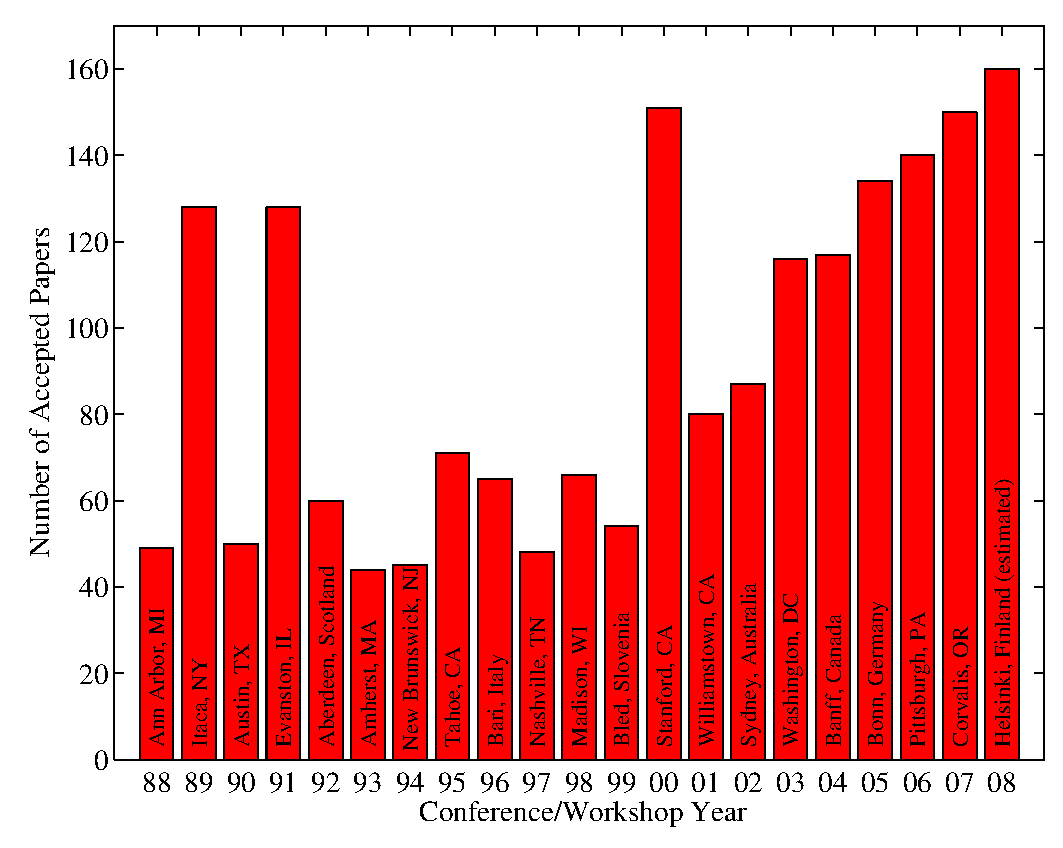
\includegraphics[width=\columnwidth]{icml_numpapers}}
\caption{Historical locations and number of accepted papers for International
Machine Learning Conferences (ICML 1993 -- ICML 2008) and International
Workshops on Machine Learning (ML 1988 -- ML 1992). At the time this figure was
produced, the number of accepted papers for ICML 2008 was unknown and instead
estimated.}
\label{icml-historical}
\end{center}
\vskip -0.2in
\end{figure}

\csubsection{Figures}

You may want to include figures in the paper to illustrate
your approach and results. Such artwork should be centered,
legible, and separated from the text. Lines should be dark and at
least 0.5~points thick for purposes of reproduction, and text should
not appear on a gray background.

Label all distinct components of each figure. If the figure takes the
form of a graph, then give a name for each axis and include a legend
that briefly describes each curve. Do not include a title inside the
figure; instead, the caption should serve this function.

Number figures sequentially, placing the figure number and caption
\emph{after} the graphics, with at least 0.1~inches of space before
the caption and 0.1~inches after it, as in
Figure~\ref{icml-historical}. The figure caption should be set in
9~point type and centered unless it runs two or more lines, in which
case it should be flush left. You may float figures to the top or
bottom of a column, and you may set wide figures across both columns
(use the environment \texttt{figure*} in \LaTeX). Always place
two-column figures at the top or bottom of the page.

\csubsection{Algorithms}

If you are using \LaTeX, please use the ``algorithm'' and ``algorithmic''
environments to format pseudocode. These require
the corresponding stylefiles, algorithm.sty and
algorithmic.sty, which are supplied with this package.
Algorithm~\ref{alg:example} shows an example.

\begin{algorithm}[tb]
   \caption{Bubble Sort}
   \label{alg:example}
\begin{algorithmic}
   \STATE {\bfseries Input:} data $x_i$, size $m$
   \REPEAT
   \STATE Initialize $noChange = true$.
   \FOR{$i=1$ {\bfseries to} $m-1$}
   \IF{$x_i > x_{i+1}$}
   \STATE Swap $x_i$ and $x_{i+1}$
   \STATE $noChange = false$
   \ENDIF
   \ENDFOR
   \UNTIL{$noChange$ is $true$}
\end{algorithmic}
\end{algorithm}

\csubsection{Tables}

You may also want to include tables that summarize material. Like
figures, these should be centered, legible, and numbered consecutively.
However, place the title \emph{above} the table with at least
0.1~inches of space before the title and the same after it, as in
Table~\ref{sample-table}. The table title should be set in 9~point
type and centered unless it runs two or more lines, in which case it
should be flush left.

% Note use of \abovespace and \belowspace to get reasonable spacing
% above and below tabular lines.

\begin{table}[t]
\caption{Classification accuracies for naive Bayes and flexible
Bayes on various data sets.}
\label{sample-table}
\vskip 0.15in
\begin{center}
\begin{small}
\begin{sc}
\begin{tabular}{lcccr}
\toprule
Data set & Naive & Flexible & Better? \\
\midrule
Breast    & 95.9$\pm$ 0.2& 96.7$\pm$ 0.2& $\surd$ \\
Cleveland & 83.3$\pm$ 0.6& 80.0$\pm$ 0.6& $\times$\\
Glass2    & 61.9$\pm$ 1.4& 83.8$\pm$ 0.7& $\surd$ \\
Credit    & 74.8$\pm$ 0.5& 78.3$\pm$ 0.6&         \\
Horse     & 73.3$\pm$ 0.9& 69.7$\pm$ 1.0& $\times$\\
Meta      & 67.1$\pm$ 0.6& 76.5$\pm$ 0.5& $\surd$ \\
Pima      & 75.1$\pm$ 0.6& 73.9$\pm$ 0.5&         \\
Vehicle   & 44.9$\pm$ 0.6& 61.5$\pm$ 0.4& $\surd$ \\
\bottomrule
\end{tabular}
\end{sc}
\end{small}
\end{center}
\vskip -0.1in
\end{table}

Tables contain textual material, whereas figures contain graphical material.
Specify the contents of each row and column in the table's topmost
row. Again, you may float tables to a column's top or bottom, and set
wide tables across both columns. Place two-column tables at the
top or bottom of the page.

\csubsection{Citations and References}

Please use APA reference format regardless of your formatter
or word processor. If you rely on the \LaTeX\/ bibliographic
facility, use \texttt{natbib.sty} and \texttt{icml2021.bst}
included in the style-file package to obtain this format.

Citations within the text should include the authors' last names and
year. If the authors' names are included in the sentence, place only
the year in parentheses, for example when referencing Arthur Samuel's
pioneering work \yrcite{Samuel59}. Otherwise place the entire
reference in parentheses with the authors and year separated by a
comma \cite{Samuel59}. List multiple references separated by
semicolons \cite{kearns89,Samuel59,mitchell80}. Use the `et~al.'
construct only for citations with three or more authors or after
listing all authors to a publication in an earlier reference \cite{MachineLearningI}.Authors should cite their own work in the third person
in the initial version of their paper submitted for blind review.

Use an unnumbered first-level section heading for the references, and use a
hanging indent style, with the first line of the reference flush against the
left margin and subsequent lines indented by 10 points. The references at the
end of this document give examples for journal articles \cite{Samuel59},
conference publications \cite{langley00}, book chapters \cite{Newell81}, books
\cite{DudaHart2nd}, edited volumes \cite{MachineLearningI}, technical reports
\cite{mitchell80}, and dissertations \cite{kearns89}.

Alphabetize references by the surnames of the first authors, with
single author entries preceding multiple author entries. Order
references for the same authors by year of publication, with the
earliest first. Make sure that each reference includes all relevant
information (e.g., page numbers).

Please put some effort into making references complete, presentable, and
consistent. If using bibtex, please protect capital letters of names and
abbreviations in titles, for example, use \{B\}ayesian or \{L\}ipschitz
in your .bib file.

\csection{Software and Data}

Importantly, all submissions must be accompanied by a GitLab hash containing the source code to reproduce all experiments in the paper. These will be manually checked by reviewers. If the grader cannot run the provided code or not all experiments are reproduced this will reduce marks from the experimental design and experimental communication sections. Additionally, if the code is missing entirely or deviates substantially from what is reported this can result in a 0 for valid experimental design. Finally, if reported results are found to be entirely fabricated the group will receive a 0 on the entire coursework and College academic honesty policies will be followed. 


% In the unusual situation where you want a paper to appear in the
% references without citing it in the main text, use \nocite
\nocite{langley00}

\bibliography{main}
\bibliographystyle{icml2021}


%%%%%%%%%%%%%%%%%%%%%%%%%%%%%%%%%%%%%%%%%%%%%%%%%%%%%%%%%%%%%%%%%%%%%%%%%%%%%%%
%%%%%%%%%%%%%%%%%%%%%%%%%%%%%%%%%%%%%%%%%%%%%%%%%%%%%%%%%%%%%%%%%%%%%%%%%%%%%%%
% DELETE THIS PART. DO NOT PLACE CONTENT AFTER THE REFERENCES!
%%%%%%%%%%%%%%%%%%%%%%%%%%%%%%%%%%%%%%%%%%%%%%%%%%%%%%%%%%%%%%%%%%%%%%%%%%%%%%%
%%%%%%%%%%%%%%%%%%%%%%%%%%%%%%%%%%%%%%%%%%%%%%%%%%%%%%%%%%%%%%%%%%%%%%%%%%%%%%%
\appendix
\csection{\emph{Do} have an appendix here}

\textbf{\emph{Feel free to put content after the references.}}
%
Feel free to add appendices to your submissions, but be aware the markers are \textit{\textbf{not}} required to consider appendicies as part of the marks for your work. 
 
%%%%%%%%%%%%%%%%%%%%%%%%%%%%%%%%%%%%%%%%%%%%%%%%%%%%%%%%%%%%%%%%%%%%%%%%%%%%%%%
%%%%%%%%%%%%%%%%%%%%%%%%%%%%%%%%%%%%%%%%%%%%%%%%%%%%%%%%%%%%%%%%%%%%%%%%%%%%%%%


\end{document}


% This document was modified from the file originally made available by
% Pat Langley and Andrea Danyluk for ICML-2K. This version was created
% by Iain Murray in 2018, and modified by Alexandre Bouchard in
% 2019 and 2021. Previous contributors include Dan Roy, Lise Getoor and Tobias
% Scheffer, which was slightly modified from the 2010 version by
% Thorsten Joachims & Johannes Fuernkranz, slightly modified from the
% 2009 version by Kiri Wagstaff and Sam Roweis's 2008 version, which is
% slightly modified from Prasad Tadepalli's 2007 version which is a
% lightly changed version of the previous year's version by Andrew
% Moore, which was in turn edited from those of Kristian Kersting and
% Codrina Lauth. Alex Smola contributed to the algorithmic style files.
